\documentclass{school-22.211-notes}
\date{April 12, 2012}

\begin{document}
\maketitle

\lecture{Exam 2 Review}
\topic{General Background}
\begin{enumerate}

\item Material $\kinf$: depend on integrated cross section only (cross sections that treat pin-cells as homogenized preserve exactly the MC fuel reactivity for infinite repeating lattices): 
  \eqn{ \kinf &= \frac{\nu \bar{\Sigma}_f }{\bar{\Sigma}_a},  
    &\kinf &= \frac{\nu \bar{\Sigma}_{f1} + \nu \bar{\Sigma}_{f2} \frac{\hat{\Sigma}_{s12} }{\bar{\Sigma}_{a2}}}{\bar{\Sigma}_{a1} + \hat{\Sigma}_{s12} }   }

\item $\keff$: take into account leakage, notice $\keff$ does not depend on volume or flux. The one group and two group expressions are, 
  \eqn{ \keff &= \frac{\nu \Sigma_f}{DB^2 + \Sigma_a}, &\kinf &= \frac{\nu \bar{\Sigma}_{f1} + \nu \bar{\Sigma}_{f2} \frac{\hat{\Sigma}_{s12} }{D_2 B^2 + \bar{\Sigma}_{a2}}}{D_1 B^2 + \bar{\Sigma}_{a1} + \hat{\Sigma}_{s12} }  } 

\item Materials bucklings,
\eqn{ B_m^2 = \frac{\frac{\nu \Sigma_f}{\keff} - \Sigma_a}{D} }
If $\keff = 1$, the material buckling is uniquely determined by the cross sections. See infinite medium critical buckling for more details. 

\item Geometrical buckling: the allowable values that satisfy the boundary conditions are uniquely determined reactor geometry. See Table~\ref{diffusion-table}. 

\item Infinite medium critical buckling: where migration area $M^2$ is a measurement of the distance travelled before absorption. 
  \eqn{ B_m^2 = \frac{\nu \Sigma_f - \Sigma_a}{D} = \frac{\frac{\nu \Sigma_f}{\Sigma_a} - 1 }{\frac{D}{\Sigma_a}} = \frac{\kinf - 1}{M^2} }

\item Divergence theorem: $\int_V (\divergence \vec{\phi} ) \dV = \int_S (\vec{\phi} \cdot \vecn) \dS$. In deriving the diffusion theorem from transport theorem, we use the divergence theorem to turn the surface integral into the volume integral,
  \eqn{ \int \vecJ \cdot \vec{n} \dS = \int \divergence \vecJ \dV }
  From there we use the Fick's law, $\vecJ = - D \gradient \phi$ to get the leakage term $-D \laplacian \phi$. 

\item Laplacian: see Table~\ref{diffusion-table}.

\item Eigenvalues/eigenfunctions: 1D multi-group diffusion equations can be written as a matrix system, and $\keff$ is the eigenvalue of the system, and the flux is the eigenfunction: 
  \eqn{ [A] [\phi] &= \frac{1}{\keff} [M] [\phi], & [A]^{-1} [M] [\phi] &= \keff [\phi] }
  If using power iteration, we solve for $[A][\phi]^{n+1} = [M] [\phi]^n$, and $\keff$ can be solved from,
  \eqn{ \keff = \frac{[M] [\phi]^{n+1} }{[M] [\phi]^n} }


\item Fission yields. General properties of fission products: most are highly unstable and rapidly decay; certain fission products are important to thermal spectrum ($\up$ thermal absorption xs, top three are: \ce{^{135} Xe}, \ce{^{103} Rh}, \ce{^{143} Nd}), but have little contribution to the fast spectrum. 
\begin{figure}[ht]
  \centering
  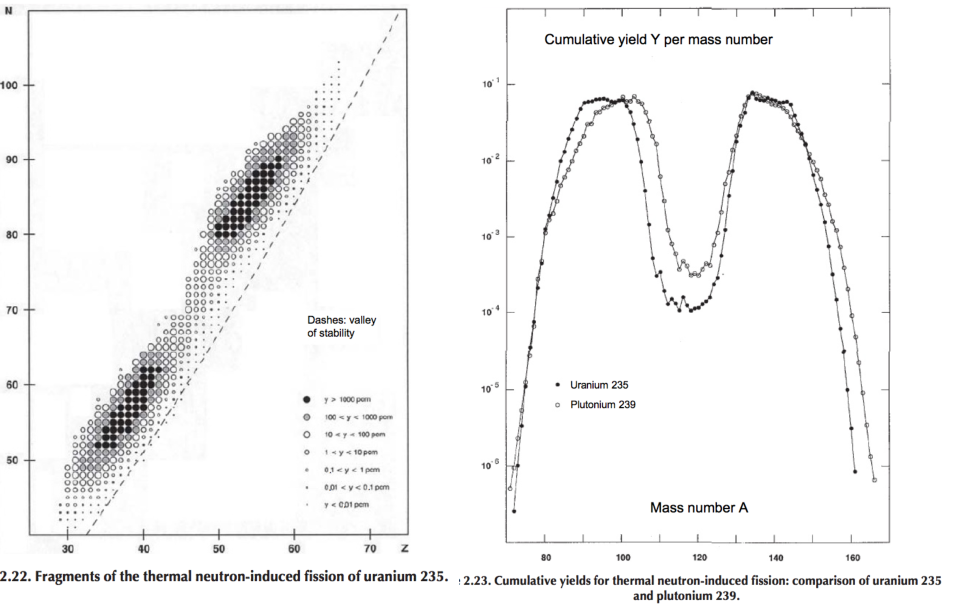
\includegraphics[width=5in]{images/dfs/fission-product-yield.png}
\end{figure}

\item Transient fission product equations: 
 \eqn{ \frac{\derivative N_i}{\dt} = \overbrace{\gamma_i \Sigma_f \phi}^{\mbox{fission gain}} - \overbrace{\lambda_i N_i}^{\mbox{decay}} - \overbrace{\sigma_i N_i \phi}^{\mbox{n capture}}  + \overbrace{ \lambda_j N_j}^{\mbox{decay of j}} + \overbrace{\sigma_k N_k \phi}^{\mbox{n capture of k}} }
 Solving the above equation, we find that: 
 \begin{itemize}
   \item Equilibrium I-135 concentration is proportional to flux: $I_{eq} = \frac{\gamma_I \Sigma_f \phi}{\gamma_I}$;
   \item Equilibrium Xe-135 concentration depends on flux at low flux, and it is independent at high flux level: $X_{eq} = \frac{(\gamma_I + \gamma_X) \Sigma_f \phi}{\gamma_X + \sigma_X \phi}$;
   \item Equilibrium Pm-149 concentration is proportional to flux: $P_{eq} = \frac{\gamma \Sigma_f \phi}{\gamma}$;
   \item Equilibrium Sm-149 concentration is independent of flux: $S_{eq} = \frac{\gamma \Sigma_f}{\sigma}$. 
 \end{itemize}

\item I/Xe, Pm/Sm reactivity effects: Xe and Sm both are fission poisoners\footnote{Xe-135 has a thermal absorption cross section of $2.6\times 10^6$ barns.}. 
\begin{itemize}
\item Major source of Xe: Iodine decay; Source of Sm: Pm decay;
\item Major sink of Xe: burnup; Sink of Sm: burnup. 
\end{itemize}
Xenon peaking happens because after shutdown, the major sink is removed, but the major source remains, hence Xenon peaks until the Iodine depletes. Reactors must be designed with enough fuel to offset the effect of Xenon. At the end of core life, there may not be enough reactivity to override peak Xenon; such reactors are called `xenon-precluded.' If a scram occurs, a restart may not be possible for 30-40 hours. See Stacy's Example 6.2 (p.214) for an example of xenon reactivity worth and illustrating diagrams. 


\begin{table}
  \centering
  \begin{tabular}{|p{0.6\textwidth}|p{0.4\textwidth}|}\hline
    \begin{minipage}[b]{0.6\textwidth}
      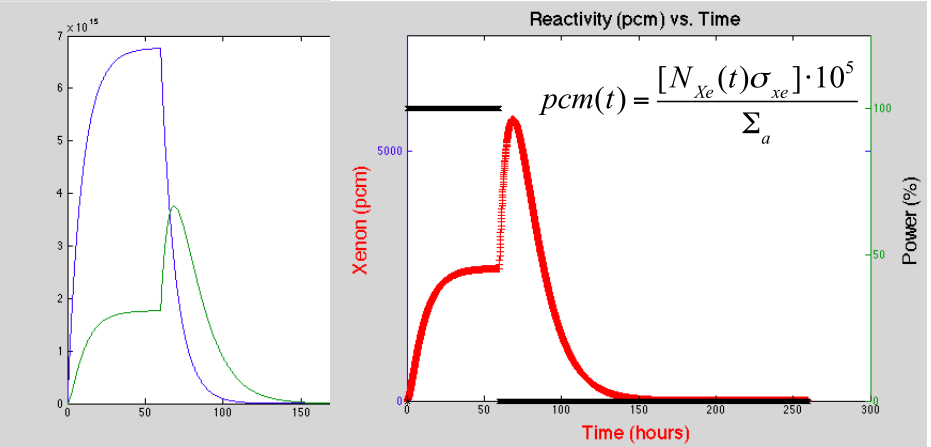
\includegraphics[width=3.5in]{images/dfs/I-Xe-1.png} 
    \end{minipage}
    & 
    \begin{minipage}[b]{0.4\textwidth}
      After startup: both I and Xe increases, and saturates after 30 hours. After shutdown: I decays quickly, whereas Xe peaks 9 hours after shutdown, and decays away in 60 hours. The peak happens because I coninues to decay into Xe, while Xe can no longer decrease through capture. 
There is a 2.5\% depress due to Xe; the higher the flux, the higher the peak is.
    \end{minipage}   \\ \hline
%
    \begin{minipage}[b]{0.6\textwidth}
      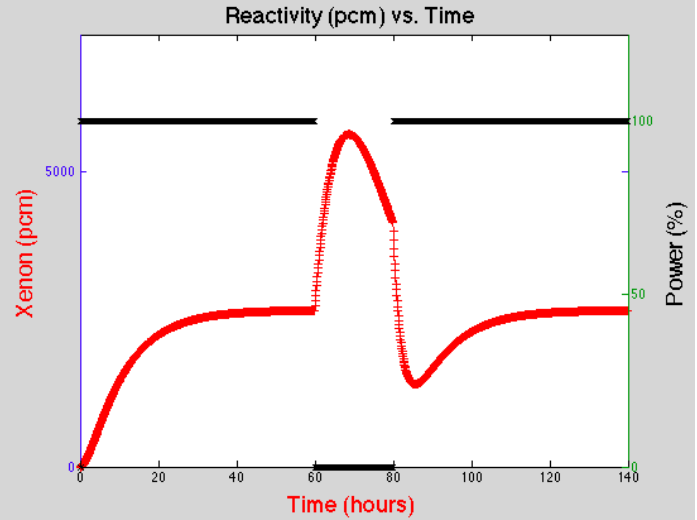
\includegraphics[width=3.5in]{images/dfs/I-Xe-2.png} 
    \end{minipage}
    & 
    \begin{minipage}[b]{0.4\textwidth}    
      A rapid startup after a scram: the concentration decreases immediately after the startup, because Xe absorption increases suddnely due to flux and the over-weight the amount from I decay. Xe would reach its equilibrium value again after about 40 hours. 
    \end{minipage}  \\ \hline
%
    \begin{minipage}[b]{0.6\textwidth}
      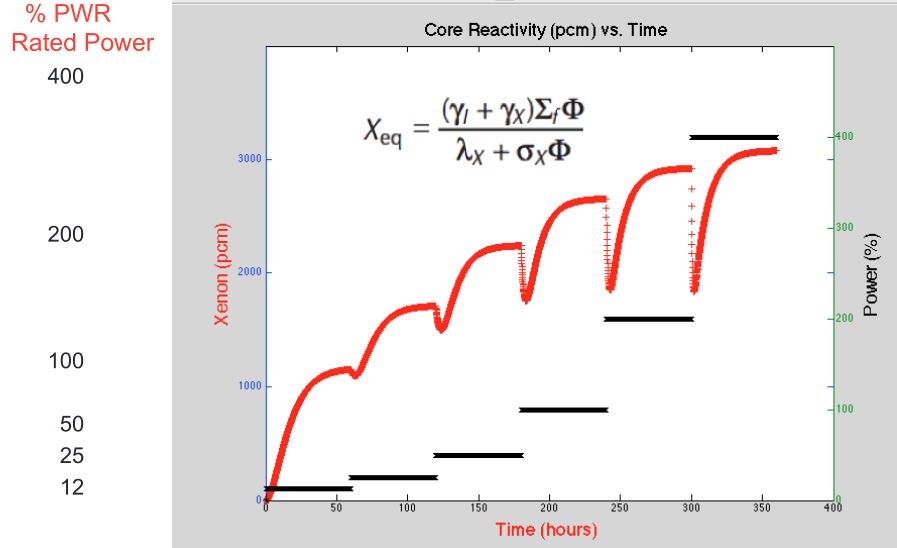
\includegraphics[width=3.5in]{images/dfs/I-Xe-3.png}
    \end{minipage}
 &  
    \begin{minipage}[b]{0.4\textwidth}    
      Equilibrium Xenon Worth: if $\phi \to \infty$, then $X_{eq}$ is independent of the flux as in the $X_{eq}$ expression; additionally, the Xenon concentration drops right after everytime power increases for the same reason as the previous case (flux increases, the destruction rate of Xe increases instantenously, but the Iodine decay rate has not increased yet). 
    \end{minipage} \\ \hline
%
    \begin{minipage}[b]{0.6\textwidth}
    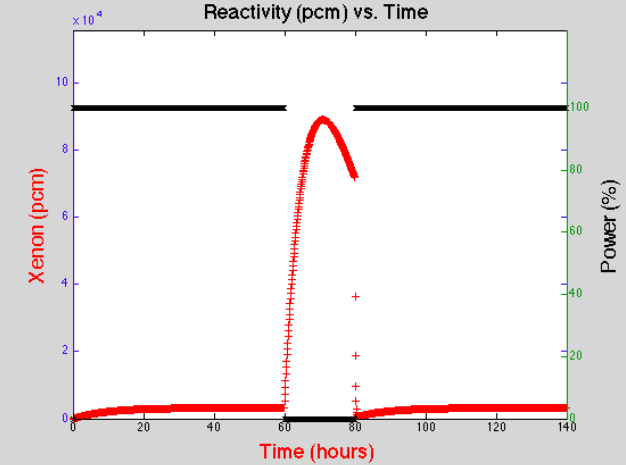
\includegraphics[width=3.5in]{images/dfs/I-Xe-4.png}
    \end{minipage}
 &  
    \begin{minipage}[b]{0.4\textwidth}
      Xenon for high flux reactor: xenon peak gives rise to a control constraint. If the reactivity reserves (control rods or poisons that can be removed) are insufficient, the reactor cannot be restarted during this period of increased xenon poisoning. We have to wait till Xe drops to re-start. Alternatively, you can start before Xenon builds up, which is pretty rare. 
      \end{minipage} \\ \hline
  \end{tabular}
\end{table}

\begin{table}
  \centering
  \begin{tabular}{|p{0.5\textwidth}|p{0.5\textwidth}|}\hline
    \begin{minipage}[b]{0.5\textwidth}
      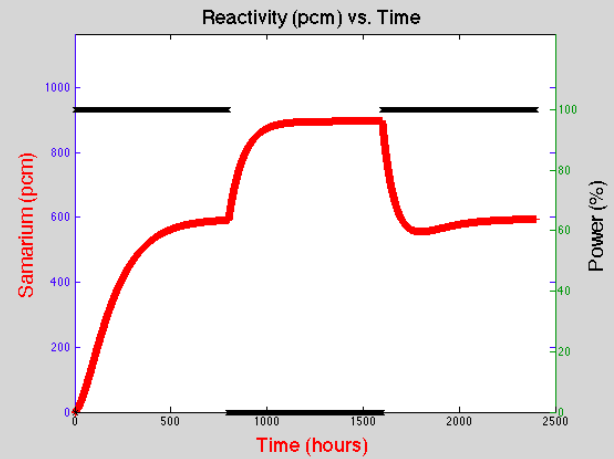
\includegraphics[width=3in]{images/dfs/Pm-Sm-1.png} 
    \end{minipage}
    & 
    \begin{minipage}[b]{0.5\textwidth}
      Pm behaves normally: it builds up and reaches equilibrium when in operation, and it decays away after shutdown. 
Sm behaves similar to Xe in the sense that both peaks after reactor shutdown (Sm peaks 200 hours after shutdown, Xe peaks 9 hours after shutdown). But Sm is stable unlike Xe, and once Pm burns out, Sm would stay constant and never decay away. Sm reactivity peaks by 200-300 pcm after shutdown. 
    \end{minipage}   \\ \hline
%
    \begin{minipage}[b]{0.5\textwidth}
      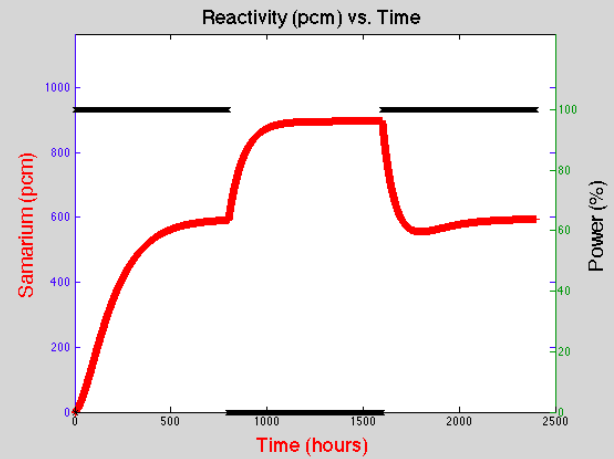
\includegraphics[width=3in]{images/dfs/Pm-Sm-2.png} 
    \end{minipage}
    & 
    \begin{minipage}[b]{0.5\textwidth}    
     Sm worth following a refueling outage: Over-write Xenon by pulling the control rods out for a couple of days; then insert the control rods for Sm. Sm returns to equilibrium about 100 hours after restart.
    \end{minipage}  \\ \hline
%
    \begin{minipage}[b]{0.5\textwidth}
      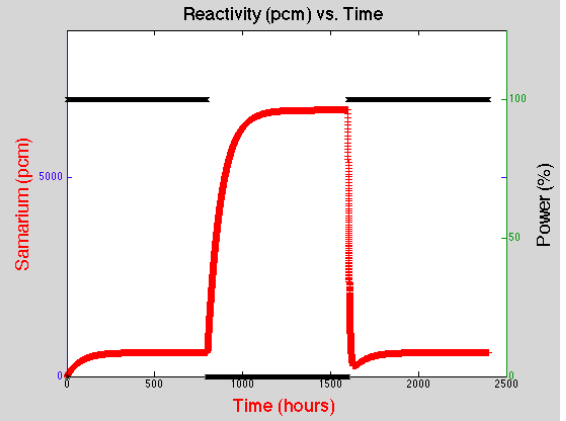
\includegraphics[width=3in]{images/dfs/Pm-Sm-3.png}
    \end{minipage}
    &  
    \begin{minipage}[b]{0.5\textwidth}    
      Sm for high flux reactor (20x PWR power density): Sm peaks a lot, which is bad because we may never be able to overrid Sm reactivity without refueling. Hence we should always have a controlled shutdown that burns out Xe/Sm before they build up. 
    \end{minipage} \\ \hline
  \end{tabular}
\end{table}
\end{enumerate}


%%%%%%%%%%%%%%%%%%%%%%%%%%%%%%%%%%%%%%%%%%%%%%%%%%%%%%%%%%%%%%%%%%%%%%%%%%%%%%%%
\clearpage
\topic{Analytical Diffusion Concepts} 
\begin{enumerate}
\item Transport cross section and diffusion coefficients: from the net current equation, assume the scattering is isotropic in the COM system, and use transport correction $P_0$ approximation, 
  \eqn{ D &= \frac{1}{3 \Sigma_{tr} }, & \Sigma_{tr} &= \Sigma_t - \Sigma_{s1} = \Sigma_t - \frac{2}{3A} \Sigma_s }

\item Effective down-scattering cross section: 
  \eqn{ \hat{\Sigma}_{s12} = \bar{\Sigma}_{s12} - \bar{\Sigma}_{s21} \frac{\phi_2}{\phi_1} }
  Typically we can assume the up-scattering is zero: $\Sigma_{s21}  = 0$.

\item Removal cross section
  \eqn{ \Sigma_{rg} = \Sigma_{tg} - \Sigma_{sgg} = \Sigma_{ag} + \Sum_{g'=1, g'\neq g}^G \Sigma_{sgg'}  }

\item Two-group diffusion equations,
  \begin{enumerate}
    \item General expression: 
      \begin{align}
        \left\{ \begin{array}{c}
          - D_1 \laplacian \phi_1 + (\Sigma_{a1} + \Sigma_{s12}) \phi_1 = \nu \Sigma_{f1} \phi_1 + \nu \Sigma_{f2} \phi_2 + S_1  \\
          - D_2 \laplacian \phi_2 + \Sigma_{a2} \phi_2 = \Sigma_{s12} \phi_1 + S_2
        \end{array} \right. 
      \end{align}

      \item Infinite medium: $\laplacian \phi \to 0$ for no leakage,
       \begin{align}
         \left\{ \begin{array}{c}
         (\Sigma_{a1} + \Sigma_{s12} ) \phi_1 = \frac{1}{\kinf} ( \nu \Sigma_{f1} \phi_1 + \nu \Sigma_{f2} \phi_2 )   \\
      \Sigma_{a2} \phi_2 = \Sigma_{s12} \phi_1
      \end{array} \right. 
         \end{align}
      \begin{align}
        \left[ \begin{array}{cc} 
            \frac{\nu \bar{\Sigma}_{f1}}{\kinf} -  \bar{\Sigma}_{a1}  - \hat{\Sigma}_{s12} & \frac{\nu \bar{\Sigma}_{f2}}{\kinf}   \\
            \hat{\Sigma}_{s12} &  - \bar{\Sigma}_{a2}  
          \end{array} \right] 
        \left[ \begin{array}{c} \phi_1 \\ \phi_2 \end{array} \right] = 0
      \end{align}

    \item Finite medium: has leakage term $DB^2$, 
       \begin{align}
         \left\{ \begin{array}{c}
           (D_1 B^2 + \Sigma_{a1} + \Sigma_{s12} ) \phi_1 = \frac{1}{\keff} ( \nu \Sigma_{f1} \phi_1 + \nu \Sigma_{f2} \phi_2 )  \\
           (D_2 B^2 +  \Sigma_{a2}) \phi_2 = \Sigma_{s12} \phi_1 
         \end{array} \right. 
       \end{align}
      \begin{align}
        \left[ \begin{array}{cc} 
            \frac{\nu \bar{\Sigma}_{f1}}{\keff} - D_1 B^2 -  \bar{\Sigma}_{a1}  - \hat{\Sigma}_{s12} & \frac{\nu \bar{\Sigma}_{f2}}{\keff}   \\
            \hat{\Sigma}_{s12} &  - D_2B^2 - \bar{\Sigma}_{a2}  
          \end{array} \right] 
        \left[ \begin{array}{c} \phi_1 \\ \phi_2 \end{array} \right] = 0
      \end{align}

\end{enumerate}

\item Multi-group diffusion equations: See Section~\ref{multi-group-diffusion}. 
\begin{align}
& - \overbrace{\int_{E_g}^{E_{g-1}} \dE \divergence D(\vecr, E) \gradient \phi(\vecr, E)}^{\mbox{leakage/diffusion term }\textcircled{1}} + 
\overbrace{\int_{E_g}^{E_{g-1}} \dE \Sigma_t(\vecr, E) \phi(\vecr, E)}^{\mbox{total interaction term }\textcircled{2}} = \overbrace{\int_{E_g}^{E_{g-1}} \dE S(\vecr, E)}^{\mbox{source term } \textcircled{3}}  \\
& + \overbrace{\int_{E_g}^{E_{g-1}} \dE \chi(E) \int_{E'} \dE' \nu \Sigma_f (\vecr, E') \phi(\vecr, E')}^{\mbox{fission source term }\textcircled{4}} 
 + \overbrace{\int_{E_g}^{E_{g-1}} \dE \int_{E'} \dE' \Sigma_s(\vecr, E'\to E) \phi(\vecr, E')}^{\mbox{scattering source term }\textcircled{5}} 
\end{align}
Cancel the within group scattering cross section and define the group-wise removal cross section, we get the final form,
\eqn{ \boxed{- \divergence D_g(\vecr) \gradient \phi_g(\vecr) + \Sigma_{rg} (\vecr) \phi_g(\vecr) = \chi_g \Sum_{g'=1}^G \nu \Sigma_{fg'} (\vecr) \phi_{g'} (\vecr) + \Sum_{g'=1,g'\neq g}^G \Sigma_{sg'g} (\vecr) \phi_{g'} (\vecr) + S_g(\vecr) } }

\item Partial currents and albedos: use $\psi = \frac{1}{4\pi} [\phi + 3 \vecOmega \cdot \vecJ]$, 
  \begin{align}
    J^+ &= \frac{1}{4} \phi + \frac{1}{2} J_n = \frac{1}{4} \phi - \frac{D}{2} \gradient \phi, & J^- &= \frac{1}{4} \phi - \frac{1}{2} J_n = \frac{1}{4} \phi + \frac{D}{2} \gradient \phi \\
    \phi &= 2[J^+ + J^-], & J_n &= J^+ - J^- =  -\frac{1}{3 \Sigma_{tr}} \gradient \phi  = - D \gradient \phi
  \end{align}
  Albedo coefficient, the coefficient of reflection, is the measurement of how much flux is reflected back: 
  \eqn{ \alpha = \frac{J^-}{J^+} = \frac{\mbox{neutrons reflected back to the core}}{\mbox{neutrons leaving the core}} }
  
\item Boundary conditions:
  \begin{enumerate}
  \item Zero flux boundary condition: $\phi(X) = 0$. 
  \item `Zero Incoming Flux' bc; if integrating over all angles in half space, it gives us `Zero Incoming Partial Current':
    \eqn{ \left. \psi(\vecr, E, \vecOmega) \right|_{\vecn \cdot \vecOmega < 0} &= 0, & J^- (\vecr_i, E) &= 0}
    There are two formulism to solve this:
    \begin{itemize}
    \item Kord's formulism: 
      \eqn{ J^- (\vecr, E) &= \frac{1}{4} \phi(\vecr, E) - \frac{1}{2} J_n (\vecr, E)  = 0, & \Aboxed{ \frac{J}{\phi} &= \frac{1}{2} } }
    \item The more conventional approach is to approximate with extropolation boundary condition: 
      \begin{align}
        J^- &= \frac{1}{4} \phi + \frac{D}{2} \gradient \phi_n \\
        \Aboxed{ \frac{\gradient \phi}{\phi} &= - \frac{1}{2D} = - \frac{3\Sigma_{tr}}{2} = - \frac{1}{d_{\mathrm{extrap}}}} 
        \mbox{   where } d_{\mathrm{extrap}} = \frac{2}{3 \Sigma_{tr}}  = \frac{2}{3} \lambda_{\mathrm{tr}}
      \end{align}
      where $D$ is the property of the material inside, and $\lambda_{tr}$ is transport mean free path. The coefficient before $\lambda_{tr}$ can be 0.711 in other formulism. 
    \end{itemize}
  \end{enumerate}

\item Interface conditions: 
  \begin{enumerate}
    \item Continuity of scalar flux: 
      \eqn{ \phi(\vecr_i^-, E) = \phi(\vecr_i^+, E) }
    \item Continuity of normal current:
      \eqn{ \vecn \cdot D(\vecr_i^-, E) \gradient \phi(\vecr_i^-, E) = \vecn \cdot D(\vecr_i^+, E) \gradient \phi(\vecr_i^+, E) }
  \end{enumerate}
\end{enumerate}


%%%%%%%%%%%%%%%%%%%%%%%%%%%%%%%%%%%%%%%%%%%%%%%%%%%%%%%%%%%%%%%%%%%%%%%%%%%%%%%%
\clearpage
\topic{Other Diffusion-Related Equations}
\begin{enumerate}
\item Balance equation derived from transport equations,
  \eqn{ \divergence \vecJ (\vecr, E) + \Sigma_t (\vecr, E) \phi(\vecr, E) = \Sum_i \int_{E'} \dE' \Sigma_s^i (\vecr, E'\to E) \phi(\vecr, E') + S_0 (\vecr, E) }
This expression is exact, because we haven't approximate $\vecJ$ yet. 

\item Using $P_1$ angular flux expansion,
  \eqn{ \psi (\vecr, E, \Omegahat) = \frac{1}{4\pi} \left[ \phi(\vecr, E) + 3 \Omegahat \cdot \vecJ(\vecr, E) \right] }
  We can get the net current equation,
  \eqn{ \frac{1}{3} \gradient \phi(\vecr, E) + \Sigma_t (\vecr, E) \vecJ(\vecr, E) = \Sum_i \int_{E'} \dE' \Sigma_{s1}^i (\vecr, E'\to E) \vecJ(\vecr, E') + \vec{S}_1(\vecr, E) }

\item From net current equation, assume no source and isotropic scattering in lab system, we can approximate the transport equation as, 
  \eqn{ \Sigma_{tr}^i (E) = \Sigma_t^i (E) - \frac{2}{3A^i} \Sigma_s^i (E) }
  Then we can solve for diffusion coefficient $D = \frac{1}{3 \Sigma_{tr}}$. 

\item Steady-state continuous energy diffusion equation:
  \eqn{ - \divergence D(\vecr, E) \gradient \phi(\vecr, E) + \Sigma_t (\vecr, E) \phi(\vecr, E) = \chi(E) \int_{E'} \dE' \nu \Sigma_f (\vecr, E') \phi(\vecr, E') + \int_{E'} \dE' \Sigma_s (\vecr, E'\to E) \phi(\vecr, E') + S(\vecr, E) }

\item One-group diffusion equation,
  \eqn{ -\divergence D(\vecr) \gradient \phi(\vecr) + \Sigma_a(\vecr) \phi(\vecr) = \frac{1}{\keff} \nu \Sigma_f(\vecr) \phi(\vecr) }

\item Helmoltz Equation: from one-group diffusion equation, we assume spatial constant cross section and use buckling term, 
  \eqn{ \laplacian \phi(\vecr) + B^2 \phi(\vecr) = 0 }
  This equation is important in showing that $\phi(\vecr)$ has a constant curvature. 
\end{enumerate}


%%%%%%%%%%%%%%%%%%%%%%%%%%%%%%%%%%%%%%%%%%%%%%%%%%%%%%%%%%%%%%%%%%%%%%%%%%%%%%%%
\clearpage
\topic{Sample Diffusion Problems}
\begin{enumerate}
\item \textbf{Homogeneous (single-region) criticality problems:}
 only the lowest node remains after the source is gone. For any positive value of material buckling, there is a unique critical size for each geometry. 
  \begin{enumerate}
  \item 1D slab $\in  \left[- \frac{L_0}{2}, \frac{L_0}{2} \right]$, no source, critical. 
    \eqn{ \dphidxn2 + B^2 \phi (x) &= 0, &\phi(x) &= A \cos (Bx) + C \sin(Bx) }
    BCs: $\phi(\pm L/2) = 0$, where $\frac{L}{2} = \frac{L_0}{2} + 0.711 \lambda_{tr}$. Two equations two unknowns, 
    \eqn{ \left[ \begin{array}{cc} \cos(BL/2) & \sin(BL/2) \\ \cos(BL/2) & -\sin(BL/2) \end{array} \right] \left[ \begin{array}{cc} A \\ C \end{array} \right] = 0 }
    Set the determinant to be zero, we get $-2 \cos (BL/2) \sin (BL/2) = 0$. There are two possibilities: 
    \eqn{ B_n&= \frac{n\pi}{L}  & \phi(x) &= \left\{ 
      \begin{array}{cc} 
        A_n \cos (B_n x) & n=1,3,5, \cdots \\
        A_n \sin (B_n x) & n=2,4,6, \cdots 
      \end{array} \right. }
    But in order for $\phi(x) \ge 0$ everywhere, only $n=1$ is possible; that is, 
    \eqn{ \phi(x) = A \cos \frac{\pi x}{L} }
    and the criticality condition implies that, 
    \eqn{ \frac{\nu \Sigma_f - \Sigma_a}{D}  = \left( \frac{\pi}{L} \right)^2 }

  \item Consider a finite cube with the dimensions $-a/2 \le x \le a/2, -b/2 \le y \le b/2, -c/2 \le z \le c/2$. The Helmholtz equation is,
    \eqn{ \pphipxn2 + \pphipyn2 + \pphipzn2 + B^2 \phi = 0}
    Assume separation of variables,
    \eqn{ \phi(x,y,z) = X(x) Y(y) Z(z) }
    \eqn{ \dXdxn2 + B_x^2 X &= 0, &\dYdyn2 + B_y^2 Y &= 0, &\dZdzn2 + B_z^2 Z &=0}
    The solution is, 
    \eqn{ \phi &= A \cos \left( \frac{\pi x}{L_x} \right)\cos \left( \frac{\pi y}{L_y} \right)\cos \left( \frac{\pi z}{L_z} \right) ,  &B^2 &= \left(\frac{\pi}{a}\right)^2 + \left(\frac{\pi}{b}\right)^2 + \left(\frac{\pi}{c}\right)^2 }


  \item Consider a finite cylinder from $-H/2$ to $H/2$ with radius $R$. We assume azmimuthal symmetry of Helmholtz Equation, 
    \eqn{\frac{1}{r} \ddr \left( r \pphipr\right) + \pphipzn2 + B^2 \phi = 0 }
    Assume separation of variables,
    \eqn{ \phi(r,z) = R(r) Z(z) }
    We plut the sepration of variables into the Helmholtz Equation, break $B^2 = B_r^2 + B_z^2$, and we get two equations one for each direction, 
    \eqn{ \frac{1}{R} \left( \dRdrn2 + \frac{1}{r} \dRdr \right) + B_r^2 = 0 }
    \eqn{ \dZdzn2 + B_z^2 Z = 0 }
    In $r$ direction, we can consider an infinite cylinder, 
    \eqn{ R(r) &= A_1 J_0 (B_r r), & B_r&= \frac{2.405}{R} }
    In $z$ direction, we can consider an infinite slab,
    \eqn{ Z(z) &= A_2 \cos(B_z z), & B_z &= \frac{\pi}{H} } 
    We combine the two directions,
    \eqn{ \phi(r,z) &= A J_0 \left( \frac{2.405}{R} r\right) \cos \left( \frac{\pi z}{H} \right), &B^2 &= B_r^2 + B_z^2 = \left( \frac{2.405}{R} \right)^2 + \left( \frac{\pi}{H} \right)^2 }
    Problems with less than one direction that is non-homogeneous can be solved this way with separation of variables.

  \item Summary for a couple of geometries
    \begin{table}[ht]
      \small
      \makebox[\textwidth][c]{
        \begin{tabular}{|l|l|l|l|} \hline
          Geometry & Diffusion Equation & Flux & Geometrical Buckling \\ \hline
          Slab $\in  \left[- \frac{L}{2}, \frac{L}{2} \right]$ &$\dphidxn2 + B^2 \phi = 0$ & $\phi = A \cos \left( \frac{\pi x}{L} \right)$ & $B^2 = \left( \frac{\pi}{L} \right)^2$ \\ 
          Sphere $\in [0, R]$  & $\dphidrn2 + \frac{2}{r} \dphidr + B^2 \phi = 0$& $\phi= \frac{A}{r} \sin \left( \frac{\pi r}{R} \right)$ & $B^2 = \left( \frac{\pi}{R} \right)^2$ \\
          Cylinder ($z: \infty$) & $\dphidrn2 + \frac{1}{r} \dphidr + B^2 \phi = 0$ & $\phi = A J_0 \left( \frac{2.405 r}{R} \right)$ & $B^2 = \left( \frac{2.405}{R} \right)^2$ \\ 
          Cylinder (z: $\pm H/2$) & $\dphidrn2 + \frac{1}{r} \dphidr + \dphidzn2 + B^2 \phi = 0$ & $\phi = A J_0\left( \frac{2.405 r}{R} \right) \cos \left( \frac{\pi z}{H} \right)$ & $B^2 = \left( \frac{2.405}{R} \right)^2 + \left( \frac{\pi}{H} \right)^2$ \\ 
          Parallelepiped ($\pm \frac{L_i}{2}$) & $\dphidxn2 + \dphidyn2 + \dphidzn2 + B^2 \phi = 0$ & $\phi = A \cos \left( \frac{\pi x}{L_x} \right) \cos \left( \frac{\pi y}{L_y} \right) \cos \left( \frac{\pi x}{L_z} \right)$ & $B^2 = \left( \frac{\pi}{L_x} \right)^2 + \left( \frac{\pi}{L_y} \right)^2 + \left( \frac{\pi}{L_z} \right)^2$ \\ \hline
        \end{tabular}
      }
      \caption{Finite Geometries With Zero Flux BC} \label{diffusion-table}
    \end{table}

  \item Find the height-to-diameter that would minimize the leakage from a fixed-volume cylinder. To minimize leakage, we need to maximize $B_m^2$ hence $B_g^2$. For a finite cylinder, we know
    \eqn{B_g^2 = \left( \frac{2.405}{R} \right)^2 + \left( \frac{\pi}{H} \right)^2 }
    and we solve $\frac{\derivative B_g^2}{\dr} = 0$. The optimal H/D ratio comes out to be 0.9236. 
    
  \end{enumerate}


\clearpage  
\item \textbf{Homogeneous (single-region) source problems:}
  \begin{enumerate}
  \item Consider a non-multiplying medium, slab geometry from $0$ to $l$, no source in the slab: 
    \eqn{ D \dphidxn2 - \Sigma_a \phi = 0 }
    The general solution is in the form of, 
    \eqn{ \phi(x) = A e^{x/L} + C e^{-x/L} = A' \sinh((l-x)/L) + C' \cosh((l-x)/L) }
    BC1: $\phi(l) = 0 \Rightarrow C' = 0$. Then we are left with, 
    \eqn{ \phi(x) = A' \sinh((l-x)/L) }
    We can find the albedo coefficient: 
    \eqn{ \alpha &= \frac{1 - \gamma}{1 + \gamma}, & \gamma &= \frac{2D}{L} \coth(l/L) }
    The parameter $\gamma$ is minus twice the current/flux ratio at the interface. The albedo improves as the thickness of the reflector increases. Eventually an asymptote is reached from a thickness of 2 or 3 $L$, 
    \eqn{ \alpha &= \frac{1 - 2D/L}{1 + 2D/L} }

  \item Consider a subcritical multiplying medium, slab geometry from $-L/2$ to $L/2$, and with a source\footnote{See Section~\ref{one-group-source-problem-subcritical}.}. 
    \begin{align}
      - D \dphidxn2 + \Sigma_a \phi(x) &= \nu \Sigma_f \phi(x) + S(x) \\
      \dphidxn2 + B_m^2 \phi(x) &= -\frac{S(x)}{D} 
    \end{align}
    Given $\Sigma_a > \nu \Sigma_f$, $B^2 = \frac{\nu \Sigma_f - \Sigma_a}{D} < 0 $, we re-write $B^2 = - |B|^2$,
    \eqn{ \dphidxn2 - |B|^2 \phi(x) = \tilde{S}(x) }
    The general/homogeneous solution is,
    \eqn{ \phi_H (x) = A e^{|B|x} + C e^{-|B|x} = A' \cosh (|B|x) + C' \sinh (|B| x) }
    The particular solution depends on source $\tilde{S}(x)$. Apply BCs $\phi \left( \pm \frac{L}{2} \right) = 0$, we get the boundary conditions in the matrix form,
    \eqn{ \left[ \begin{array}{cc} 
          \cosh(|B|L/2) & \sinh(|B|L/2) \\
          \sinh(|B|L/2) & \cosh(|B|L/2) 
        \end{array} \right] 
      \left[ \begin{array}{c}
          A' \\ C' \end{array} \right] 
      = - \left[ \begin{array}{c} 
          \phi_p(L/2) \\ \phi_p(-L/2) \end{array} \right] }
    The coefficients are uniquely determined for a given source distribution: 
    \begin{itemize}
    \item There always exists a physically realizable solution (no critical buckling!);
    \item In the limit of $S\to 0$, the only physical solution is the trivial solution. 
    \end{itemize}



    \clearpage
  \item Conside an infinite non-multiplying medium with a point source. 
    \eqn{ \dphidrn2 + \frac{2}{r} \dphidr - \ols\phi = -\frac{S_0}{D} \delta(\vecr) }
    We look for the homogeneous solution, and set $w = r \phi$, 
    \eqn{ \dphidrn2 + \frac{2}{r} \dphidr - \ols\phi &= 0, &\dwdrn2 - \ols w &= 0}
    The solution is, 
    \eqn{ w &= Ae^{r/L} + B e^{-r/L}, & \phi(r) = A\frac{e^{r/L}}{r} + B \frac{e^{-r/L}}{r} }
    BC1: $\lim_{r\to \infty} \phi = 0, \Rightarrow A=0$. BC2: $\lim_{r\to 0} 4 \pi r^2 J(r) = S_0$ (specific solution), that is, 
    \begin{align}
      J &= -D \dphidr = DBe^{-r/L} \left( \frac{1}{r^2} + \frac{1}{rL} \right), 
      &\lim_{r\to 0} 4 \pi r^2 J(r) &= 4 \pi DB = S_0 \\
      B &= \frac{S_0}{4 \pi D}, & \phi(r) &= \frac{S_0}{4\pi D} \frac{e^{-r/L}}{r} 
    \end{align}

  \item Consider an infinite non-multiplying medium with a line source along the z-axis. Use cylindrical coordinates, only $\rho$ is involved:
    \eqn{ D\left[ \frac{\dphi^2}{\derivative^2 \rho} + \frac{1}{\rho} \frac{\dphi}{\drho} \right] - \ols \phi = - \frac{S}{D} }
    The solution is in terms of Bessel functions, 
    \eqn{ \phi(\rho) = A K_0(\rho/L) + B I_0(\rho/L) }
    BC1: $\lim_{\rho \to \infty} \phi = 0, \Rightarrow B = 0$, BC2: $\lim_{\rho \to 0} 2 \pi J = S$, that is, 
    \eqn{ \phi(\rho) = \frac{S}{2\pi D} K_0(\rho/L) }


  \item Consider an infinite non-multiplying medium with a plane source at $x=0$. Since the geometry is symmetric, we can solve for $x>0$ first. 
    \eqn{ \phi(x) = Ae^{x/L} + B e^{-x/L}} 
    BC1: $\lim_{x \to \infty} \phi(x) = 0, \Rightarrow \phi(x) = B e^{-x/L}$; BC2: $\lim_{x\to 0} J(r)  = \frac{S_0}{2}$, 
    \eqn{ J = -D \dphidx = B D e^{-x/L} }
    \eqn{ \phi(x) = \frac{S_0 L}{2D} e^{-x/L}}
    For the total geometry, we can simply place an absolute sign on $x$:
    \eqn{ \phi(x) = \frac{S_0 L}{2D} e^{-|x|/L}}
    If the source is placed at $x=b$, the solution becomes,
    \eqn{ \phi(x) = \frac{S_0 L}{2D} e^{-|x-b|/L} } 

  \item Consider a finite multiplying medium with $\kinf > 1$, it is a slab extending from $-H/2$ to $H/2$, it is subcritical with leakage, BC are from the current at center and the zero flux at the H/2 boundary. 
    \eqn{ \dphidxn2 + B_m^2 \phi &= 0,  & B_m^2 &= \frac{\nu \Sigma_f - \Sigma_a}{D} = \frac{\kinf - 1}{L^2} > 0}
    \eqn{ \phi(x) = A \cos(B_mx) + B\sin(B_mx) }
    BC1: $\phi(H/2) = 0$; BC2: $J(0) = \frac{S_0}{2}$. We can solve for the coefficients, and place absolute sign to represent the whole geometry: 
    \eqn{ \phi(x) = \frac{S_0}{2DB_m \cos\left( \frac{B_m H}{2} \right)} \sin\left[ B_m \left(\frac{H}{2} - |x|\right) \right] }
    \begin{figure}
      \centering
      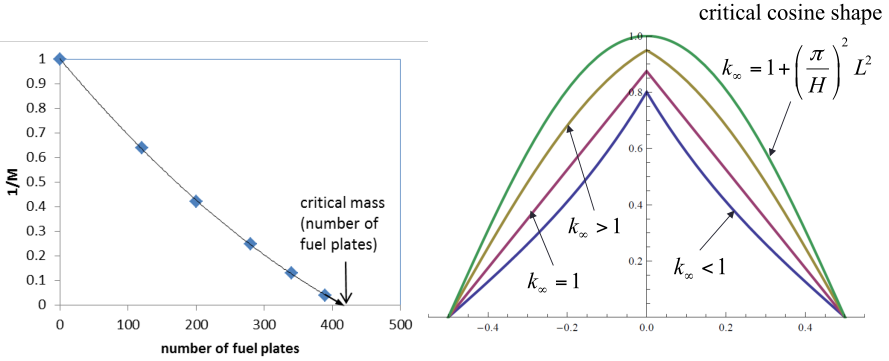
\includegraphics[width=5in]{images/dfs/approach-critical.png}
    \end{figure}

    \item Consider a finite multiplying medium with $\kinf < 1$, a slab geometry from $0$ to $H$, and a plane source at $0$, 
      \eqn{ B_m^2 = \frac{\nu \Sigma_f - \Sigma_a}{D} &= \frac{k_{\infty} - 1}{L^2} < 0, & B_m^2 &\to -|B_m|^2}
      The homogeneous solution is, 
      \eqn{\dphidxn2 - |B_m|^2 \phi &= 0, &\phi(x) &= A\cosh(|B_m|x) + B \sinh(|B_m|x) }
      BCs: $\phi(0) = \phi_0, \phi(H) = 0$, we can solve for the coefficients, 
      \eqn{ \phi(x) = \phi_0 \left[ \cosh(|B_m|x) - \frac{\cosh(|B_m|x)}{\sinh(|B_m|x)} \sinh(|B_m|x) \right] }
  \end{enumerate}

\clearpage  
\item Multi-region diffusion problems
\begin{enumerate}
\item Consider a critical reflected slab reactor in the following image. 
  \begin{figure}[ht]
    \centering
    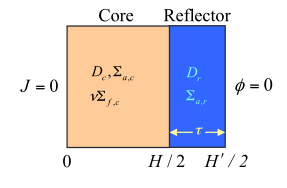
\includegraphics[width=2in]{images/dfs/reflected-slab.png}
  \end{figure}
  \eqn{-D^c \laplace \phi^c + \Sigma_a^c \phi^c &= \frac{1}{\keff} \nu \Sigma_f^c \phi^c,  &-D^r \laplace \phi^r + \Sigma_a^r \phi^r &= 0 }
  \eqn{ B^2 &= \frac{\frac{\kinf}{\keff} - 1}{L_c^2}, & \kappa^2 &= \frac{1}{L_r^2} = \frac{\Sigma_a^r}{D^r} = -B_{m,r}^2 }
  \eqn{ \laplace \phi^c + B^2 \phi^c &= 0, &\laplace \phi^r - \kappa^2 \phi^r &= 0}
  The solutions are in the forms of,
  \eqn{ \phi^c(x) &= C_1 \cos(Bx) + C_2 \sin(Bx), &\phi^r(x) &= C_3 \cosh(\kappa x) + C_4 \sinh (\kappa x) }
  BC1: reflective boudnary condition at $x=0$, BC2: zero flux at reflector surface, 
  \eqn{ J^c(0) &= 0 \Rightarrow C_2 = 0, & \phi(H'/2) &= 0 \Rightarrow C_3 = 0} 
  We have: 
  \eqn{ \phi^c (x) &= C_1 \cos (Bx), & \phi^r (x) &= C_4' \sinh[\kappa(H'/2 - x)] }
  Apply two interface conditions: 
  \eqn{ \phi^c (H/2) &= \phi^r (H/2), & J^c(H/2) &= J^r (H/2) }
  which can be written in the matrix form, 
  \begin{align}
    \left[ \begin{array}{cc}
        \cos (BH/2) & -\sinh(\kappa \tau) \\
        D^c B \sin(BH/2) & -D^r \kappa \cosh(\kappa \tau) 
      \end{array} \right] 
    \left[ \begin{array}{c} 
        C_1 \\ C_4' \end{array} \right] = 0
  \end{align}
  We define the reflector thickness $\tau = \frac{H' - H}{2}$, then the coefficients can be solved,
  \eqn{ C_1 &= \phi^c (0), & C_4' &= C_1 \frac{\cos (BH/2)}{\sinh(\kappa \tau) } }
  which gives us the criticality condition,
  \eqn{ D^c B \tan \left(\frac{B H}{2} \right) = D^r \kappa \coth (\kappa \tau) }
  Interpretation:
  \begin{enumerate}
  \item Since $B$ is defined with $\keff$, 
    \eqn{ B^2 = \frac{\frac{\kinf}{\keff} - 1}{L^2} }
    we need to satisty an expression between $\keff$ and $H$. We can either,
    \begin{enumerate}
    \item Given $H$, search for the $\keff$ that satisfies the equivalence;
    \item Given $\keff$, search for the $H$ that satisfies the equivalence,
      \eqn{H = \frac{2}{B_m} \tan^{-1} \left[ \frac{D^r \kappa}{D^c B_m} \coth (\kappa \tau) \right] }
      That is, as $H \down, \tau \up$. For large $\tau$, like $\kappa \tau > 3, \coth (\kappa \tau) \to 1$, the smallest $H$ to reach criticality is,
      \eqn{H = \frac{2}{B_m} \tan^{-1} \left[ \frac{D^r \kappa}{D^c B_m} \right] }
    \end{enumerate}
  \item Critical dimension is reduced by the presence of the reflector: 
    \eqn{   s = \frac{\tilde{H}}{2} - \frac{H}{2}   = \frac{1}{B_m} \left\{ \frac{\pi}{2} - \tan^{-1} \left[ \frac{D^r \kappa}{D^c B_m} \coth(\kappa \tau) \right] \right\} }
    \eqn{   \tan\left[ \frac{\pi}{2} - \tan^{-1} x \right] &= \cot [\tan^{-1} x ] = \frac{1}{\tan[\tan^{-1} x]} = \frac{1}{x}, & \frac{\pi}{2} - \tan^{-1} x &= \tan^{-1} \left( \frac{1}{x} \right) }
    \eqn{  \Aboxed{ s &= \frac{1}{B_m} \tan^{-1} \left[ \frac{D^c B_m}{D^r \kappa} \tanh(\kappa \tau) \right] } }
  \item For larger cores, $B_m \to 0$ and $\tan^{-1} x \approx x $, that is, 
    \eqn{ s = \frac{D^c}{D^r \kappa} \tanh(\kappa \tau) = \frac{D^c}{D^r} L^r \tanh\left( \frac{\tau}{L^r} \right)  }
    That is, 
    \begin{align}
      \left\{ \begin{array}{ccc} 
        \tau \ll L^r & s \approx \frac{D^c}{D^r} \tau &  (\tanh x \approx x \mbox{ for }x\ll 1) \\
        \tau \gg L^r & s \approx \frac{D^c}{D^r} L^r &  (\tanh x \approx 1 \mbox{ for }x > 3) 
      \end{array} \right. 
    \end{align}
  \end{enumerate} % end of two-region slab problem



\end{enumerate} % end of multi-region diffusion problem
\end{enumerate} % end of practise problems


%%%%%%%%%%%%%%%%%%%%%%%%%%%%%%%%%%%%%%%%%%%%%%%%%%%%%%%%%%%%%%%%%%%%%%%%%%%%%%%%
\clearpage
\topic{Numerical Diffusion Theory}
\begin{enumerate}
\item Finite-difference diffusion equation: 
  \begin{enumerate}
  \item Interface flux: 
    \eqn{J_n^+ &= - \hat{D}^{n,n+1} (\phi^{n+1} - \phi^n)  & J_n^- &= - \hat{D}^{n-1, n} (\phi^n - \phi^{n-1} ), & \hat{D}^{n,n+1} &= \frac{2 D^n D^{n+1}}{\Delta (D^n + D^{n+1})}   }

  \item Finite-difference equation: 
    \begin{align*}
      - \hat{D}_1^{n-1,n} \phi_1^{n-1} - \hat{D}_1^{n,n+1} \phi_1^{n+1} + [ \Sigma_{r1}^n \Delta^n + \hat{D}_1^{n-1, n} + \hat{D}_1^{n,n+1} ] \phi_1^n 
      &= \nu \Sigma_{f1}^n \phi_1^n \Delta^n + \nu \Sigma_{f2}^n \phi_2^n \Delta^n + S_1^n \Delta^n \\
      - \hat{D}_2^{n-1,n} \phi_2^{n-1} - \hat{D}_2^{n,n+1} \phi_2^{n+1} + [\Sigma_{a2}^n \Delta^n + \hat{D}_2^{n-1.n} + \hat{D}_2^{n,n+1} ] \phi_2^n 
      &= \Sigma_{s12}^n \phi_1^n \Delta^n + S_2^n \Delta^n 
    \end{align*}

  \item BC: 
    \begin{align}
      \mbox{Zero Flux BC:} & J_g^N = -D_g^N \frac{ -\phi_g^N - \phi_g^N}{\Delta^N}  = \frac{2 D_g^N}{\Delta^N} \phi_g^N \\
      \mbox{Zero Incoming Flux BC:} & J_g^N = \frac{2D_g^N}{\Delta^N} \left[ \frac{1}{1 + \frac{4 D_g^N}{\Delta^N}} \right] \phi_g^N 
    \end{align}

    \item Matrix form: 
      \begin{align}
        \left[ \begin{array}{cc} 
            [L_1 + D_1 + U_1] & [0] \\
            -[T_2] & [L_2 + D_2 + U_2] \\
          \end{array} \right] 
        \left[ \begin{array}{c}
            \phi_1 \\ \phi_2 \\ \end{array} \right] 
        = \left[ {\begin{array}{cc} \left[M_1\right] & \left[M_2\right] \\ \left[0\right] & \left[0\right] \end{array}} \right] 
        \left[ \begin{array}{c}
            \phi_1 \\ \phi_2 \\ \end{array} \right] 
        + 
        \left[ \begin{array}{c} 
            S_1 \\ S_2 \\ \end{array} \right] 
      \end{align}
      Whose compressed form is, 
      \eqn{ [A] [\phi] = [M] [\phi] + [S] }
\end{enumerate}


\item Fission source iterations: the equation we are trying to solve is,
\eqn{ [A] [\phi]^{n+1} &= [M] [\phi]^n }
An initial guess of the flux $\phi_i^{(0)}$ at each point and of the eigenvalue $\lambda^{(0)}$ is made and an initial fission source at each point is constructed $S_i^{(0)} = M \phi_i^{(0)}$. The Gaussian elimination is performed to determine $\phi_i^{(1)} = A^{-1} S_i^{(0)}$. Then we update the source term as well based on the flux. A new estimate of the eigenvalue is made from: 
\eqn{ \keff = \frac{S_i^{(1)}}{S_i^{(0)}} }
The process is continued until the eigenvalues obtained on two successive iterates differ by less than a threshold level. The rate our fission source converges depends on material, geometry etc.

\item Gauss-Jacobi flux inner iterations: 
\begin{figure}[ht]
  \centering
  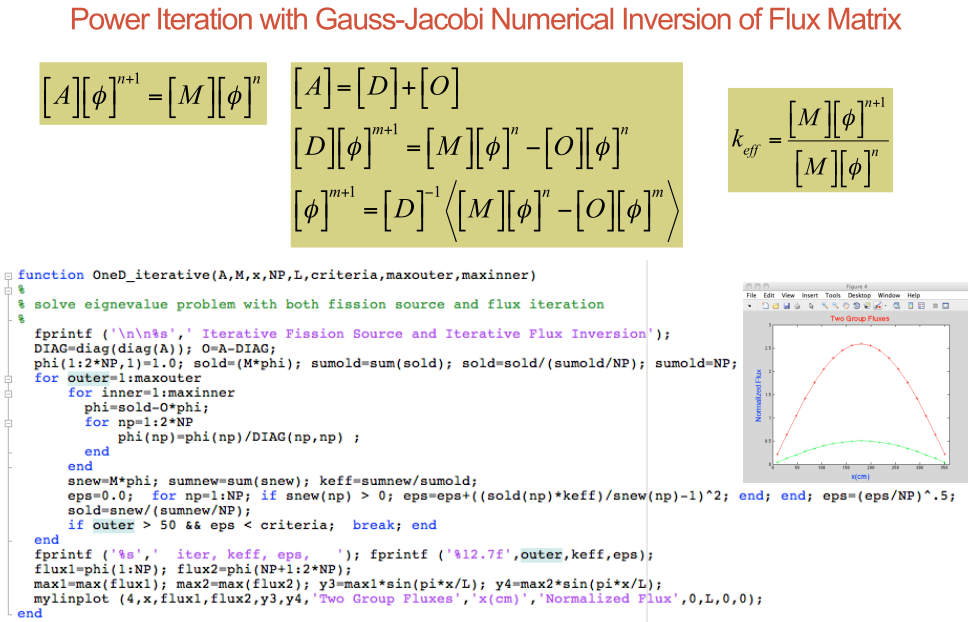
\includegraphics[width=5in]{images/dfs/power-iteration-Gauss-Jacobi.png}
\end{figure}

\item Dominance ratio estimation: 
Given an eigenvalue problem, if we specify the solved eigenvalues to be:
\eqn{ |\lambda_1| > |\lambda_2| \ge |\lambda_3| \ge \cdots }
then $|\lambda_1|$ is the spectral radius of the iteration matrix, and every mode has a dominance ratio,
\eqn{ \dr_n = \frac{\lambda_n}{\lambda_1} }
and power iteration kills of the lowest dominance ratio modes. The last remaining mode is the fundamental mode $dr = \frac{\lambda_2}{\lambda_1}$. If $|\lambda_1| \ge 1$, the ietration scheme is unstable and it would not converge. Convergence of the power method is slow when $d$ is close to unity; in fact in most numerical methods, convergence rate = 1 - dominance ratio.

Dominance ratio measures the spatial decoupling, and it depends on: symmetric mode, core size (size $\up$, $\dr \up$, takes longer), decoupling of the radial zones, and of the axial zones. 

\item Order of operations (not included in official list): Matrix inversion is of $N^3$, finding all eigenvalues is at least $N^2$, iterative inversion must be order $N$ to be practical, multi-level iteration is a necessity. 
\end{enumerate}

\clearpage
\topic{Appendix A: Finite Difference 1D Transport Equation}
In this chapter we are doing a fine-mesh finite difference (example: PDQ, CITATION). 

\subtopic{Deriving Balance Equation}
Start from neutron balance equation derive the finite-difference form of it. Note: we omit the $\chi_g$ term but it could be there. 

\begin{align}
\divergence J_g(x) + \Sigma_{t,g} \phi_g(x) &= \Sum_{k=1}^{G} \Sigma_{s,kg} \phi_k (x) + \frac{1}{k} \Sum_{k=1}^{G} \nu \Sigma_{f,kg} \phi_k(x) \\
\frac{\dJ_g}{\dx} + \Sigma_{t,g} \phi_g(x) &= \Sum_{k=1}^{G} \Sigma_{s,kg} \phi_k (x) + \frac{1}{k} \Sum_{k=1}^{G} \nu \Sigma_{f,kg} \phi_k(x) 
\end{align}
We define the removal term,
\eqn{ \frac{\dJ_g}{\dx} + \overbrace{(\Sigma_{tg} - \Sigma_{s,gg})}^{\Sigma_{rg}} \phi_g(x) -  \Sum_{k=1, k\neq g}^{G} \Sigma_{s,kg} \phi_k (x) &= \frac{1}{k} \Sum_{k=1}^{G} \nu \Sigma_{f,kg} \phi_k(x)  }
Then we can discritize the domain into the following (insert image). 

We make assumptions,
\begin{itemize}
\item All groups are spatially constant of a computational cell; 
\item Average flux equals flux at the center of a cell;
\item First order approximation on $\dphidx$ (linear that is);
\end{itemize}

Integrate over an arbitrary cell, 
\eqn{ \int_{i-1/2}^{i+1/2} \frac{\dJ_g}{\dx} \dx + \int_{i-1/2}^{1/2} \Sigma_{rg} \phi_g(x) \dx - \int_{i-1/2}^{i+1/2} \Sum_{k=1,k\neq g}^{G} \Sigma_{s,kg} \phi_k (x) &= \frac{1}{k}\int_{i-1/2}^{i+1/2} \Sum_{k=1}^{G} \nu \Sigma_{f,kg} \phi_k(x)  }
\begin{enumerate}
\item The leakage term: 
  \eqn{ \int_{i-1/2}^{i+1/2} \frac{\dJ_g}{\dx} \dx = J_g^{i+1/2} - J_g^{i-1/2} }
\item First we find the exact expression for the volume-averaged flux in each cell: 
  \eqn{ \overline{\phi}_g^i = \frac{\int_{i-1/2}^{i+1/2} \phi_g(x) \dx}{\Delta x_i} }
Then we make a second-order approximation, 
\eqn{ \overline{\phi}_g^i &= \phi_g^i = \int_{i-1/2}^{i+1/2} \phi_g(x) \dx = \phi_g^i \Delta x_i }
\end{enumerate}
Then we have,
\eqn{ J_g^{i+1/2} - J_g^{i-1/2} + \Sigma_{rg}^i \phi_g^i\Delta x_i - \Sum_{k=1,k\neq g}^G \Sigma_{s,kg}^i \phi_k^i \Delta x_i = \frac{1}{k} \Sum_{k=1}^G \nu \Sigma_{f,kg}^i \phi_k^i \Delta x_i }
\eqn{\boxed{ \frac{J_g^{i+1/2} - J_g^{i-1/2}}{\Delta x_i} + \Sigma_{rg}^i \phi_g^i - \Sum_{k=1,k\neq g}^G \Sigma_{s,kg}^i \phi_k^i  = \frac{1}{k} \Sum_{k=1}^G \nu \Sigma_{f,kg}^i \phi_k^i} }
Notice here if we were to expand 1D into 3D, we need to add two more leakage terms making a total of six net current terms. 

\clearpage
\subtopic{Computing Interface Current}
Insert boundary image here. Then we can write the net current at the boundary two different ways, 
\eqn{ J_g^{i+1/2} = - D_g^i \left. \dphidx \right|_{i+1/2} \approx -D_g^i \left( \frac{\phi_g^{i+1/2} - \phi_g^i}{\Delta x_i /2} \right) }
\eqn{ J_g^{i+1/2} = - D_g^{i+1} \left. \dphidx \right|_{i+1/2} \approx -D_g^{i+1} \left( \frac{\phi_g^{i+1} - \phi_g^{i+1/2}}{\Delta x_{i+1} /2} \right) }
and set the above two expressions to be the same, we can hence solve for the interface current, 
\begin{align}
 -D_g^i \left( \frac{\phi_g^{i+1/2} - \phi_g^i}{\Delta x_i /2} \right) & =  -D_g^{i+1} \left( \frac{\phi_g^{i+1} - \phi_g^{i+1/2}}{\Delta x_{i+1} /2} \right) \\
\phi_g^{i+1/2} &= \frac{D_g^i \Delta x_{i+1} \phi_g^i + D_g^{i+1} \Delta x_i \phi_g^{i+1}}{D_g^i \Delta x_{i+1} + D_g^{i+1} \Delta x_i} 
\end{align}
Plug the interface flux into either expression for the interface net current, we get, 
\begin{align}
 J_g^{i+1/2} &= - \frac{2D_g^i}{\Delta x_i} \left( \frac{D_g^i \Delta x_{i+1} \phi_g^i + D_g^{i+1} \Delta x_i \phi_g^{i+1}}{D_g^i \Delta x_{i+1} + D_g^{i+1} \Delta x_i}  - \phi_g^i \right) \\
&= - \frac{2D_g^i}{\Delta x_i} \left( \frac{D_g^i \Delta x_{i+1} \phi_g^i + D_g^{i+1} \Delta x_i \phi_g^{i+1} - D_g^i \Delta x_{i+1} \phi_g^i - D_g^{i+1} \Delta x_i \phi_g^i }{D_g^i \Delta x_{i+1} + D_g^{i+1} \Delta x_i} \right) \\
&= - \frac{2D_g^i}{\Delta x_i} \left( \frac{D_g^{i+1} \Delta x_i \phi_g^{i+1} - D_g^{i+1} \Delta x_i \phi_g^i }{D_g^i \Delta x_{i+1} + D_g^{i+1} \Delta x_i} \right) \\
\Aboxed{ J_g^{i+1/2} &= - \frac{2D_g^i D_g^{i+1}}{D_g^i \Delta x_{i+1} + D_g^{i+1} \Delta x_i} (\phi_g^{i+1} - \phi_g^i) = - \tilde{D}_g^{i+1/2} (\phi_g^{i+1} - \phi_g^i) }
\end{align}
Similarly, we can construct the net current on the left hand side, 
\eqn{ J_g^{i-1/2} &= - \frac{2D_g^{i-1} D_g^{i}}{D_g^{i-1} \Delta x_{i} + D_g^{i} \Delta x_{i-1}} (\phi_g^{i} - \phi_g^{i-1}) = - \tilde{D}_g^{i-1/2} (\phi_g^{i} - \phi_g^{i-1}) }


\clearpage
\subtopic{Deriving the Matrix Form}
Substuite the interface current term into the balance equation, we get an all-flux-equation,
\eqn{  - \frac{\tilde{D}_g^{i+1/2}}{\Delta x_i} (\phi_g^{i+1} - \phi_g^i)
+ \frac{\tilde{D}_g^{i-1/2}}{\Delta x_i} (\phi_g^i - \phi_g^{i-1}) 
 + \Sigma_{rg}^i \phi_g^i - \Sum_{k=1,k\neq g}^G \Sigma_{s,kg}^i \phi_k^i  = \frac{1}{k} \Sum_{k=1}^G \nu \Sigma_{f,kg}^i \phi_k^i }
Rearranging,
\eqn{\boxed{  - \frac{\tilde{D}_g^{i+1/2}}{\Delta x_i} \phi_g^{i+1} 
+ \left( \frac{\tilde{D}_g^{i+1/2}}{\Delta x_i} + \frac{\tilde{D}_g^{i-1/2}}{\Delta x_i} + \Sigma_{rg}^i \right) \phi_g^i
- \frac{\tilde{D}_g^{i-1/2}}{\Delta x_i} \phi_g^{i-1}
 - \Sum_{k=1,k\neq g}^G \Sigma_{s,kg}^i \phi_k^i  = \frac{1}{k} \Sum_{k=1}^G \nu \Sigma_{f,kg}^i \phi_k^i } }
\eqn{ [M] [\phi] &= \frac{1}{k} [F] [\phi] }
\begin{itemize}
\item The generalized eigenvalue problem is $F\phi = k M \phi$. If using solver, solving the generalized eigenvalue problem is faster than the eigenvalue problem. 
\item The eigenvalue problem is $M^{-1} F \phi = k \phi$. Notice we need to re-arrange the matrix form to the eigenvalue form to get that $k$ is the eigenvalue. Also keep in mind that $[F]$ can be singular, so we try to avoid inverting $[F]$ whenever possible. 
\end{itemize}
Keep in mind it is always column impact rows. 
The above expression is true all the time; with different BC, the coupling coefficients (the $\tilde{D}$ terms) would change\footnote{these coupling terms couple the interface current to the cell-averaged fluxes}. Next we will investigate the different boundary conditions. 
\begin{enumerate}
\item Zero Flux BC: 
  \eqn{ J_g^{I+1/2} = - D_g^I \left. \dphidx \right|_{I+1/2} \approx -D_g^I \frac{\overbrace{\phi_g^{I+1/2}}^{\to 0} - \phi_g^I}{\Delta x_I/2} = \frac{2D_g^I}{\Delta x_I} \phi_g^I = \tilde{D}_g^{I+1/2} \phi_g^I }
\item Reflective Flux BC:
  \eqn{ J_g^{I+1/2} = 0 }
\item Vacuum BC (Zero Incoming Flux BC): 
  \eqn{ J_g&= (J_g^+ - J_g^-) \cdot \vecn}
  From Mashek BC from transport theory, we know,
  \eqn{ J_g^+ &= \frac{1}{4} \phi_g + \frac{1}{2} J_g \cdot \vecn, & J_g^- &= \frac{1}{4} \phi_g - \frac{1}{2} J_g \cdot \vecn }
  The convention is that $J_g^-$ is the incoming current for both surfaces. Then for vaccum BC, we set $J_g^- = 0$, that is, $J_g^{I+1/2} = \frac{1}{2} \phi_g^{I+1/2}$. 
  \begin{align}
    J_g^{I+1/2} &= - D_g^I \left( \frac{\phi_g^{I+1/2} - \phi_g^I}{\Delta x_I/2} \right) \\
    &= - \frac{2D_g^I}{\Delta x_i} (\phi_g^{I+1/2} - \phi_g^I) \\
    &= - \frac{2D_g^I}{\Delta x_i} (2J_g^{I+1/2} - \phi_g^I) \\
    J_g^{I+1/2}&= \frac{2D_g^I}{\Delta x_I + 4D_g^I} \phi_g^I \\
    &= \tilde{D}_g^{I+1/2} \phi_g^I 
  \end{align}
\end{enumerate}

\begin{algorithm}
  \begin{algorithmic}
    \FOR {every cell}
    \STATE irow = $i$ + $nx(g-1)$;
    $i$ = mod(irown, $nx$) + 1;
    $g$ = mod(irow, $nx \cdot ny$)/$nx$ + 1;
    \ENDFOR
  \end{algorithmic}
  \caption{Index Scheme}
\end{algorithm}


%%%%%%%%%%%%%%%%%%%%%%%%%%%%%%%%%%%%%%%%%%%%%%%%%%%%%%%%%%%%%%%%%%%%%%%%%%%%%%%%
\clearpage
\topic{Appendix B: Math Reviews}
\begin{enumerate}
\item Trigonometry:
 \begin{align}
  \sin(x) &= \mathrm{Im}(e^{ix}) = \frac{e^{ix} - e^{-ix}}{2i} & \cos(x) &= \mathrm{Re}(e^{ix})\frac{e^{ix} + e^{-ix}}{2} \\
  \sin(ix) &= -i \sinh(x) & \cos(ix) &= \cos (x) \\
  e^{\pm ix} &= \cos(x) \pm i\sin(x) 
\end{align}


\item Hyperbolic functions:
\begin{align}
  \sinh(x) &= \frac{e^x - e^{-x}}{2} & \cosh(x) &= \frac{e^x + e^{-x}}{2} \\
  \sinh(x) &= -i \sin(ix) & \cosh(x) &= \cos (ix)  \\
  e^{\pm x} &= \cosh(x) \pm \sinh(x)
\end{align}

\begin{figure}[ht]
  \centering
  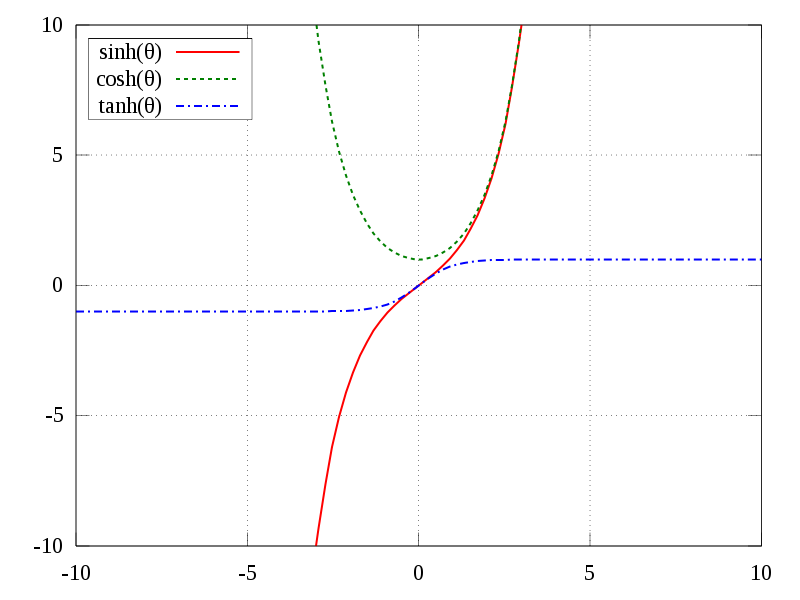
\includegraphics[width=4in]{images/dfs/sinh-cosh.png}
\end{figure}

\end{enumerate}


\end{document}
